\documentclass[a4paper]{article}

% Character encoding and font
\usepackage[utf8]{inputenc}
\usepackage[T1]{fontenc}
\usepackage{textcomp}

% Page layout
\usepackage[a4paper]{geometry}

% Math and symbols
\usepackage{amsmath}
\usepackage{amssymb}
\usepackage{amsthm}
\usepackage{bm}

% Graphics and colors
\usepackage{graphicx}
\usepackage{color}
\usepackage{tikz}
\usetikzlibrary{graphs} 

% Tables and formatting
\usepackage{booktabs}
\usepackage{empheq}
\usepackage{mdframed}
\usepackage{enumitem}

% Miscellaneous
\usepackage{standalone}

% Custom colors
\definecolor{matteOrange}{RGB}{255,179,71} % A matte orange color
\definecolor{deepGreen}{RGB}{26,111,0}
\definecolor{shallowGreen}{RGB}{235,255,255}
\definecolor{deepBlue}{RGB}{61,124,222}
\definecolor{shallowBlue}{RGB}{235,249,255}

% Required packages for the new box style
\usepackage{tcolorbox}

\usepackage[utf8]{inputenc}

% Default fixed font does not support bold face
\DeclareFixedFont{\ttb}{T1}{txtt}{bx}{n}{8} % for bold
\DeclareFixedFont{\ttm}{T1}{txtt}{m}{n}{8}  % for normal

% Custom colors
\usepackage{color}
\definecolor{deepblue}{rgb}{0,0,0.5}
\definecolor{deepred}{rgb}{0.6,0,0}
\definecolor{deepgreen}{rgb}{0,0.5,0}

\usepackage{listings}

% Python style for highlighting
\newcommand\pythonstyle{\lstset{
language=Python,
basicstyle=\ttm,
morekeywords={self},              % Add keywords here
keywordstyle=\ttb\color{deepblue},
emph={MyClass,__init__},          % Custom highlighting
emphstyle=\ttb\color{deepred},    % Custom highlighting style
stringstyle=\color{deepgreen},
commentstyle=\footnotesize\rmfamily\color{deepgreen}, % non-italic and small comments
frame=tb,                         % Any extra options here
showstringspaces=false
}}


% Python environment
\lstnewenvironment{python}[1][]
{
\pythonstyle
\lstset{#1}
}
{}

\newcommand\pythoninline[1]{{\pythonstyle\lstinline!#1!}}

% New orangebox command
\newcommand\orangebox[1]{%
	\begin{tcolorbox}[
		enhanced,
		arc=7pt, % Curved corners
		boxrule=1pt, % Border thickness
		colback=matteOrange, % Background color
		colframe=black, % Border color
		fontupper=\normalfont, % Text font
		parbox=false, % Allows for multi-line content
		boxsep=5pt, % Inner padding
		left=10pt, % Left padding
		right=10pt, % Right padding
		top=5pt, % Top padding
		bottom=5pt, % Bottom padding
	]
	#1
	\end{tcolorbox}
}
\newcommand{\ttl}[2]{\begin{center}\Large\textbf{#1}\end{center}\vspace{2mm}}
\newcommand{\ct}[1]{~\cite{#1}}

% List settings
\setlist[itemize]{noitemsep}
\setlist[enumerate]{noitemsep}

% Figure support
\usepackage{import}
\usepackage{xifthen}
\usepackage{pdfpages}
\usepackage{transparent}
\newcommand{\incfig}[1]{%
	\def\svgwidth{\columnwidth}
	\import{./figures/}{#1.pdf_tex}
}

% PDF settings
\pdfminorversion=7
\pdfsuppresswarningpagegroup=1


\begin{document}

\ttl{Using MUS for SMART++}

SMART generates new assertions in blocks.
Assertions are represented by the set, $A$.
Blocks are provided with some varible set that is a subset of all variables
present in the traces.

\[ 
\hat{V} \subseteq V 
\]

Each block contains a number of threads that recived a subset of $\hat{V}$
and produces a single assertion.
Currently $\hat{V}$ is generated randomly from $V$.
The idea is to use the Minimal Universal Subset, $MUS$, 
to guide in the varibales to be included in future $\hat{V}$s. 


\section*{Preliminaries}

\subsubsection*{MUS and MSA}

Exhaustative methods of finding the $MUS$ are expensive,
so we propose an approximate method that returns a set, $N$, 
for which every variable in $N$ is underspecified, formall;

\begin{equation}\label{eq:mus}
N = \{\, v \in V \mid \exists (V \setminus N) \;.\; \forall N \;.\; A \,\}
\end{equation}

There exists some assignments to all varaibles not in $N$
such that $A$ is true for any assignment to varibales in $N$,
suggesting that variables in $N$ are underspecified.
This is not $MUS$ as it makes no claim to $N$ being minimal.
Note that the $MUS$ is the dual of  Minimal Satisfying Assignments, $MSA$,
a minimal parital assignment of variables in $A$ such that $A$ is always true.

\[
MSA = (M, \sigma) . A
\]
where $(M, \sigma)$ is a partial assignemnt to $V$,
$M$ is a model and $\sigma$ is a mapping from
variables to the assigment.

\subsubsection*{MHS}

A Minimal Hitting Set ($MHS$) of a $A$
is a minimal subset of $V$ such that for each assertion, $a \in A$, 
some variable of $a$ is in the $MHS$.

\[
MHS = \{ T \subseteq V \mid \forall a \in A \;. \; T \cap a \;.\; \not = \emptyset  \}	
\]

We can generate an approximate $MHS$ for $A$ as follows;

\begin{python}
def approx_MHS(AV, V, T={}): 
"""
 AV: List of sets of variables in each assertion in A
 T:  A potentially non-empty set of variables we think we want to include 
"""
  uncovered = V
  sorted_vars = vars_by_count(AV) 
  while is_uncovered(AV):
    next_v = sorted_vars.pop(0)
    T.add(next_v)
    uncovered = {x for x in uncovered if next_v not in x}
  return T
\end{python}

We will say that an (approx) $MHS$ covers $A$ if 
$V \setminus MHS$ is an $MUS$ (the $MHS$ is an approx $MSA$).


%==================================================
\section*{Algorithm}
%==================================================

Give a set $A$ of assertions, the algorithm to get an approximate MUS proceeds as follows:

We search for an approx MSA
by starting with an approximate MHS~.
This is a good starting point, 
given the each assertion in $A$ is true,
we know that our MSA must hit each assertion with
at least one varaible. 

Partial assignemnt to the the variables in the $MHS$ 
is usually not sufficient to ensure $A$ is true for all 
assignemnts to variables in $V \setminus MHS$
and hence we need to add variables to the $MHS$ until it covers $A$.
This is described in the following pseudocode:

\begin{python}
def search(AV, V, A, its):
  mhss = [approx_MHS(AV)]
  msa_sets = []
  for _ in range(its):
    mhs = mhss.pop()
    if is_mus(V/mhs, A): 
	  # Optional: decend_to_boundary(mhs, V, A)
      msa_sets.append(mhs)
    else:
      msa = ascend_to_boundary(mhs, V, A)
      msa_sets.append(msa)
      # initialise new mhs by starting with unsatisfiable vars from previous candidate
      mhss.append(approx_mhs(AV, mhs-msa))
  return msa_sets
\end{python}

To check whether $V \setminus MHS$ is an $MUS$ (and hence $MHS$ is an $MSA$)
 we use the query described in equation \ref{eq:mus}
by calling to an SMT sovler (usually CVC5).
We make this more efficient by storing previously tested candidates, $C$.
Given some new $MUS$ query, $q$ there are three possibilities:
\begin{enumerate}
\item If $\exists c \in \{c \in C \mid \text{ismus}(c) \}  \mid q \subseteq c$ 
then $q$ is also $MUS$
\item If $\exists c \in \{c \in C \mid \neg \text{ismus}(c) \}  \mid c \subseteq q$ 
then $q$ is not an $MUS$
\item Otherwise; test using CVC5 and store in $C$ as appropriate
\end{enumerate}

If the $MHS$ is not an $MSA$ we introduce more variables from $V$ until
it covers $A$.
To be more targetted with how we add variables, 
we attempt to extract an unsat core from our $MUS$ query, $q$,
and add those varaibles to the $MHS$.
However, querying with quantifiers stops us being able to automatically extracting this from CVC5.
Instead we overapproximate the unsat core by checking for each assertion in $A$,
if the relavent variables in $q$ are not underspecified.

\begin{python}
def approx_unsatcore(q, A):  # q is a set of, potentially MUS,  variables
  specified = {}
  for a in A:
    q_p = {v for v in a if a in q}
    if q_p.issubet(specified):
      continue
    if not is_mus(q_p, a):
      specified = specified.union(q_p)
  return specified
\end{python}

This is used in \pythoninline{ascend_to_boundary} to get an approximate $MSA$:

\begin{python} 
def ascend_to_boundary(MSA, V, A):
  specified_vars = approx_unsatcore(V/MSA)
  return MSA.union(specified_vars)
\end{python}

The final idea is to use the \verb|unsat_vars| to guide the generation 
of the next $MHS$ that we propose as a candidate $MSA$.
We know that this set of variables need to be specified
for some subset of the assertions.
However, this is an overapproximation of the variables as there may be redundency between them,
given that we check an assertion at a time not the whole set $A$ together,
and that these variables were unsat given the specific $MHS$.

Doing so may arise in scenarios where our $MHS$ is an $MSA$, 
including redundant variables.
For this we can, optionally, \pythoninline{descend_to_boundary};
where we greedily remove each variable until we reach the boundary where 
the candidate is no longer an $MSA$.

\begin{python}
def descend_to_boundary(q, V, A):
  for v in q:
    q_p = q/{v}
    if not is_mus(V/q_p, A)
      return q

\end{python}


\subsection*{More traces}

When we find a valid $MUS$ we 
get a subset, $N$, of $V$ that is underspecified,
but we also get an assignment for $V \setminus N$ 
that models the hardware, given $A$.
The idea is to use this assignment and 
test if it is a positive or negative trace;
\begin{enumerate}
\item If it is positive, add it to the positive traces and continue
\item If it is negative, add it to the negative traces and re-run the block with the same
variable set, $\hat{V}$, given this new negative trace.
\end{enumerate}
This should further ensure we are generating good asseritons, 
increasing mutation detection.


\section*{Engineering}

This method works but is compute heavy for large $A$.
This is due to the SMT query and the large search space when ascending/descending.
Thus to effectively integrate this into SMART++ we can use the following structure;

\begin{enumerate}
\item Generate assertions for all variables in $V$
  \begin{itemize}
  \item Split $V$ into $n$ independent sets, each sent to a block
  \item This returns an independent set of assertions $A_i$
  \item For each $A_i$ we generate $mus_i$
  \item After $n$ blocks we generate $MUS$ from $\bigcup_{i=1}^n mus_i$
  \end{itemize}
\item Given all variables are covered in $\bigcup_{i=1}^n A_i$
  \begin{itemize}
  \item Split $MUS$ into $n$ independent sets, each sent to a block
  \item continue as above
  \end{itemize}
\end{enumerate}

This improves the efficiency of $MUS$ calculation as we can run it 
on subsets of $A$. 
And we are still able to capture variables dependecies through
iterative $MUS$ generation and refinement.

\begin{figure}
\centering
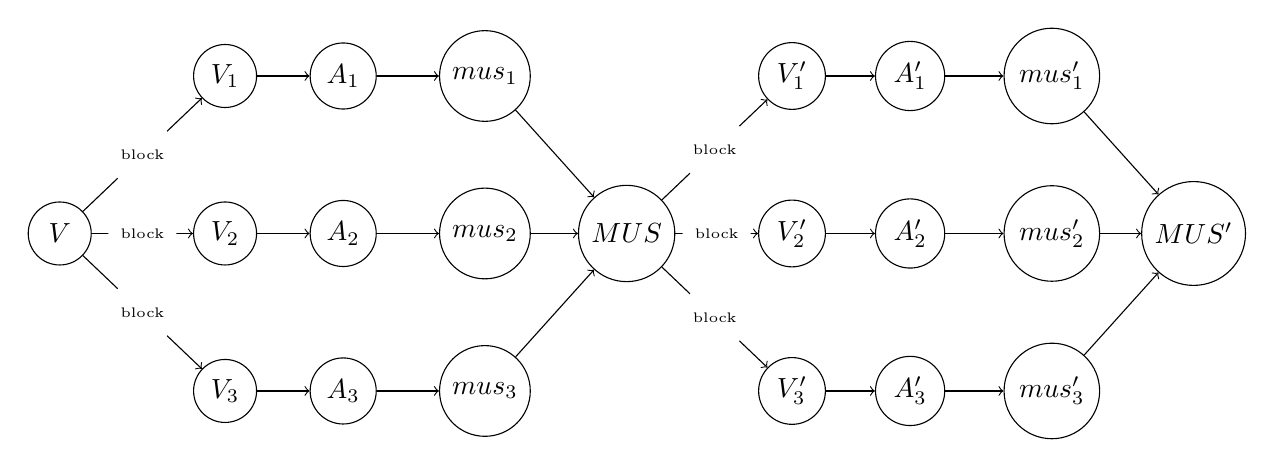
\begin{tikzpicture}[
  node distance=1.5cm and 2.5cm,
  every node/.style={draw, circle, minimum size=0.8cm},
  every edge quotes/.style={draw=none, fill=none, font=\small}
]
  % First column
  \node (V) at (0,0) {$V$};
  
  % Second column
  \node (V1) at (2.1,2) {$V_1$};
  \node (V2) at (2.1,0) {$V_2$};
  \node (V3) at (2.1,-2) {$V_3$};
  
  % Third column
  \node (A1) at (3.6,2) {$A_1$};
  \node (A2) at (3.6,0) {$A_2$};
  \node (A3) at (3.6,-2) {$A_3$};
  
  % Fourth column
  \node (mus1) at (5.4,2) {$mus_1$};
  \node (mus2) at (5.4,0) {$mus_2$};
  \node (mus3) at (5.4,-2) {$mus_3$};
  
  % Fifth column
  \node (MUS) at (7.2,0) {$MUS$};
  
  % Sixth column
  \node (V1p) at (9.3,2) {$V'_1$};
  \node (V2p) at (9.3,0) {$V'_2$};
  \node (V3p) at (9.3,-2) {$V'_3$};
  
  % Seventh column
  \node (A1p) at (10.8,2) {$A'_1$};
  \node (A2p) at (10.8,0) {$A'_2$};
  \node (A3p) at (10.8,-2) {$A'_3$};
  
  % Eighth column
  \node (mus1p) at (12.6,2) {$mus'_1$};
  \node (mus2p) at (12.6,0) {$mus'_2$};
  \node (mus3p) at (12.6,-2) {$mus'_3$};
  
  % Ninth column
  \node (MUSp) at (14.4,0) {$MUS'$};
  
  % Arrows
  \foreach \i in {1,2,3} {
  \draw[->] (V) -- node[midway, draw=none, fill=white] {\tiny block} (V\i);
  \draw[->] (V\i) -- (A\i);
  \draw[->] (A\i) -- (mus\i);
  \draw[->] (mus\i) -- (MUS);
  \draw[->] (MUS) -- node[midway, draw=none, fill=white] {\tiny block} (V\i p);
  \draw[->] (V\i p) -- (A\i p);
  \draw[->] (A\i p) -- (mus\i p);
  \draw[->] (mus\i p) -- (MUSp);
  }
\end{tikzpicture}
\end{figure}

\end{document}
